%%%%%%%%%%%%%%%%%%%%%%%%%%%%%%%%%%%%%%%%%%%%%%%%%%%%%%%%% 
% LaTeX Beamer Presentation
%
% Theme: Madrid (as requested)
%
% FIX: Implemented automatic Table of Contents display at the 
%      beginning of each defined section using \AtBeginSection.
%%%%%%%%%%%%%%%%%%%%%%%%%%%%%%%%%%%%%%%%%%%%%%%%%%%%%%%%%

\documentclass{beamer}

\mode<presentation>
{
  % --- THEME: Using the robust Madrid theme as requested. ---
  \usetheme{Madrid}
  
  % --- TEMPLATE SETTINGS ---
  \setbeamertemplate{navigation symbols}{} % Hides navigation buttons
  % Now uses the Madrid default footline.


}

% Setting Logo in every slide
% \logo{
\includegraphics[width=.1\textwidth]{../figures/AIIIMA.jpeg}}
% --- Setting the acronyms
\usepackage[nolist]{acronym}
\begin{acronym}
  \acro{SLR}[SLR]{Systematic Literature Review}
  \acro{PICOC}[PICOC]{Population, Intervention, Comparison, Outcome,
    Context}
  \acro{DL}[DL]{Deep Learning}
  \acro{AI}[AI]{Artificial Intelligence}
  \acro{BC}[BC]{Breast Cancer}
  \acro{MLO}[MLO]{Medio Lateral Oblique}
  \acro{MG}[MG]{Mammography}
  \acro{CADe}[CADe]{Computer-Aided Detection}
  \acro{CADx}[CADx]{Computer-Aided Diagnosis}
  \acro{MIAS}[MIAS]{Mammographic Image Analysis Society}
  \acro{ZSL}[ZSL]{Zero-Shot Learning}
  \acro{SAM}[SAM]{Segment Anything Model}
  \acro{MedSAM}[MedSAM]{MedSAM}
  \acro{OOD}[OOD]{out-of-domain}
  \acro{HITL}[HITL]{Human-in-the-Loop}
\end{acronym}


% --- AUTOMATIC TOC AT BEGINNING OF EACH SECTION ---
\AtBeginSection[]
{
  \begin{frame}
    \frametitle{Presentation Outline}
    \tableofcontents[currentsection] % Only shows the current section/subsection list
  \end{frame}
}

% --- PACKAGES ---
\usepackage[utf8]{inputenc}
\usepackage{graphicx}      % For images
\usepackage{booktabs}      % For professional tables
\usepackage{amsmath}       % For math
\usepackage{amssymb}       % For math
\usepackage{xcolor}        % Keeping xcolor for the custom teal color
% in the bar chart
\usepackage{array}           % For extended table functionality
\usepackage{tabularx}
\usepackage{multirow}        % For multirow cells
\usepackage[autolanguage]{numprint}
\usepackage[style=ieee,backend=biber]{biblatex}
\addbibresource{../bibliography.bib} % your .bib file


\definecolor{myteal}{RGB}{17, 202, 160} % Keeping only the necessary color definition

% --- PRESENTATION METADATA ---
\title[SAM \& Otsu in  MG Segmentation]{
  Towards a segmentation of the pectoral muscle and masses present in mammograms by combining modern and traditional techniques
}
\author[Falconi, et al.]{
  Lenin G. Falconi \inst{1} \and
  Maria Pérez \inst{1} \and
  Monserrate Intriago-Pazmiño{1} \and \\
  Aura Conci \inst{2}
}
\institute[EPN \and UFF]{
  \inst{1} Escuela Politécnica Nacional, Quito, Ecuador \\
  \inst{2} Instituto de Computação, Universidade Federal Fluminense, Brazil
}
\date[CSCI 2025]{The 2025 International Conference on Computational
  Science and Computational Intelligence}

% --- DOCUMENT START ---
\begin{document}

% \titlegraphic{
%   
\includegraphics[width=1.5cm]{../figures/AIIIMA.jpeg}
% }

% --- SLIDE 1: TITLE PAGE ---
\begin{frame}
  \titlepage
\end{frame}

% Table of Contents
\begin{frame}
    \frametitle{Overview}
    \tableofcontents
\end{frame}
% ===================================
% SECTION 1: INTRODUCTION
% ===================================
\section{Introduction}

% --- SLIDE 2: THE CHALLENGE ---

\subsection{Problem Statement and Motivation}

\begin{frame}[allowframebreaks]
  \frametitle{The importance of Segmentation in Breast Cancer}
  \begin{columns}[T]
    % Column 1
    \begin{column}{0.48\textwidth}

        \begin{itemize}
          \item \ac{BC} is a  leading cause of mortality among women worldwide.
          \item Early detection is  essential to improve  patient survival rates.
          \item Accurate image segmentation in \ac{MG} is fundamental for the
            identification of pathologies.
        \end{itemize}

    \end{column}
    % Column 2
    \begin{column}{0.48\textwidth}
      \begin{figure}[ht]
        \centering
        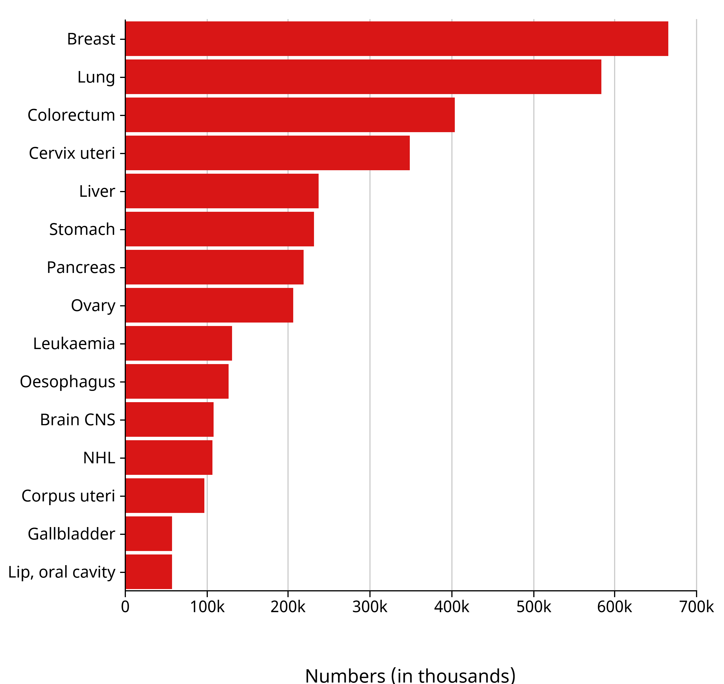
\includegraphics[width=\textwidth, height=.6\textheight]{./figures_ppt/BreastCancerFacts.png}
        \caption{\label{}https://gco.iarc.who.int/today }
      \end{figure}
    \end{column}
  \end{columns}
\end{frame}

\begin{frame}
  \frametitle{Problem Statement}
  \begin{itemize}
    \item Pectoral muscle pixels exhibit high intensity, similar to glandular tissue, leading to false positives in \ac{CADe} systems.
    \item Pectoral muscle morphology varies significantly across patients.
    \item Manual identification of abnormalities in \ac{MG} is time-consuming for radiologists.
    \item Labeled data for pectoral muscle segmentation is scarce.
    \item Expert labeling is expensive and time consuming.
  \end{itemize}
\end{frame}

\begin{frame}
  \frametitle{Problem Statement}
  \begin{figure}[ht]
    \centering
    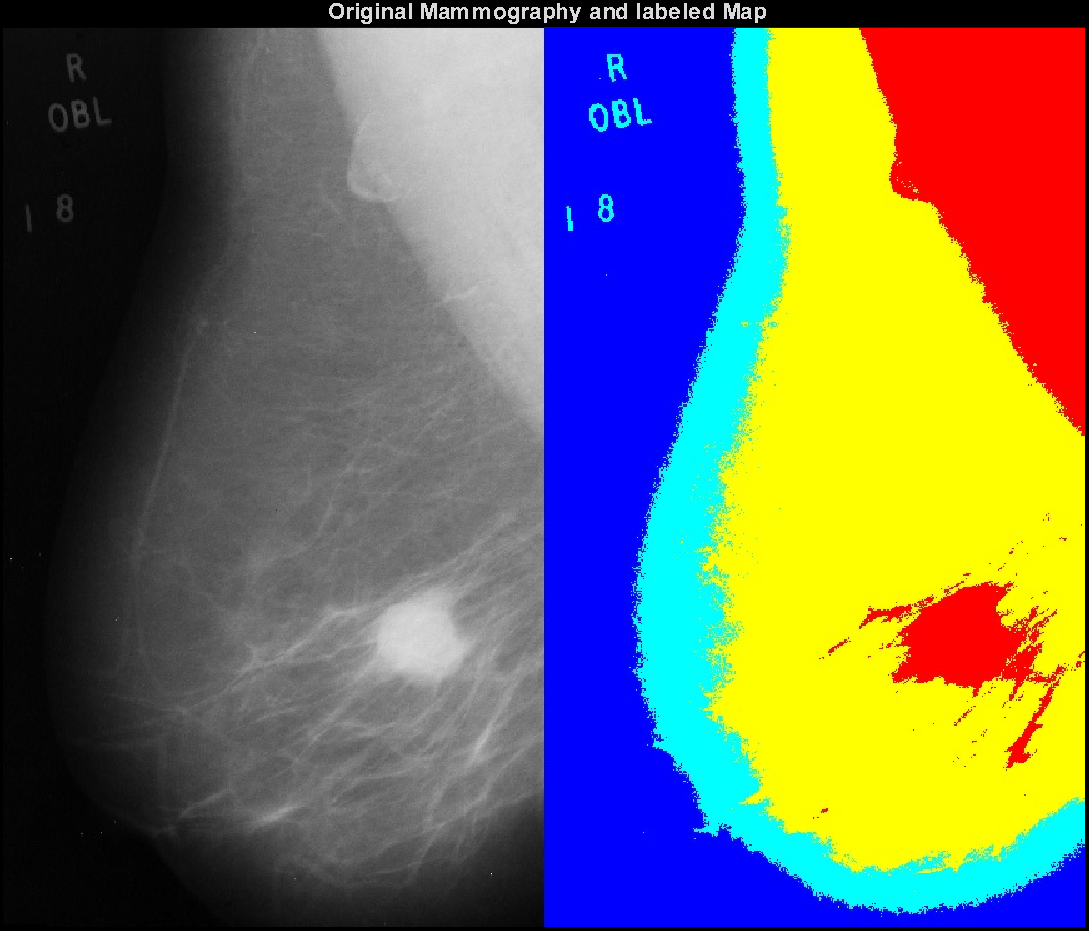
\includegraphics[width=\textwidth, height=.6\textheight]{./figures_ppt/pectoralMuscleProblem.pdf}
    \caption{\label{fig:label}Segmentation Map }
  \end{figure}

\end{frame}


% --- SLIDE 3: PROPOSED ALTERNATIVE ---

\subsection{Research Questions}
\begin{frame}
  \frametitle{Research Questions and Objectives}
  \begin{itemize}
    \item Given the strong \ac{OOD} generalization of foundational
      models, can they perform accurate pectoral muscle segmentation
      in a \ac{ZSL} setting with a human in the loop in a \ac{MG}?
    \item How does \ac{MedSAM} perform in pectoral muscle segmentation under \ac{ZSL} conditions?
    \item Do traditional segmentation approaches retain relevance for this specific task?
    % \item Would a hybrid approach, combining foundational and traditional methods, yield superior performance?
  \end{itemize}
\end{frame}
\subsection{Contribution}


% --- SLIDE 4: THE CORE PROBLEM ---
\begin{frame}
  \frametitle{Paper Contributions}
  \begin{enumerate}
    \item Performance assessment of \ac{MedSAM} in pectoral muscle segmentation using \ac{ZSL} with a human-in-the-loop approach.
    \item A manual segmentation pipeline to enhance the \ac{MG} and its borders.
    \item A Pectoral Muscle Segmentation Dataset.
    \item An iterative Otsu algorithm for automatic segmentation of the \ac{MG}.
  \end{enumerate}
\end{frame}
\section{Basic Concepts}

\subsection{Otsu Algorithm}
\begin{frame}[allowframebreaks]
  \frametitle{Otsu Algorithm}
  \begin{itemize}
  \item Classical, non-parametric, and unsupervised thresholding
    algorithm for automatic image segmentation.
  \item It determines an optimal threshold value to separate pixels
    into foreground and background classes by maximizing the
    between-class variance in the image histogram
  \end{itemize}
For an image with grayscale levels \( L \) (typically 0-255), let:
\begin{itemize}
    \item $n_i$ be the \textbf{number of pixels} at intensity level $i$, where $i \in [0, L-1]$.
    \item  $N$ be the \textbf{total number of pixels} in the image.
    \item The \textbf{probability} $p_i$ of a randomly selected pixel having intensity $i$ is given by:
    \[
    p_i = \frac{n_i}{N}
    \]
    This defines the normalized histogram, or the \emph{probability mass function (PMF)} of the image intensities.
\end{itemize}

The algorithm searches for a threshold \( k \) that divides pixels into two classes:
\begin{itemize}
    \item \textbf{Class $C_0$}: Pixels with intensities in the range $[0, k]$
    \item \textbf{Class $C_1$}: Pixels with intensities in the range $[k+1, L-1]$
\end{itemize}

The optimal threshold \( k^* \) is found by maximizing:

\[
\sigma_B^2(k) = \omega_0(k) \cdot \omega_1(k) \cdot [\mu_0(k) - \mu_1(k)]^2
\]

where:
\begin{itemize}
    \item The cumulative probability for class $C_0$ at threshold $k$ is defined as:
    \[
    \omega_0(k) = \sum_{i=0}^{k} p_i
    \]
    where $p_i$ is the probability of intensity level $i$.

    \item The cumulative probability for class $C_1$ is the complement:
    \[
    \omega_1(k) = \sum_{i=k+1}^{L-1} p_i = 1 - \omega_0(k)
    \]
    where $L$ is the total number of discrete intensity levels.

    \item The mean intensity for class $C_0$, given threshold $k$, is:
    \[
    \mu_0(k) = \frac{1}{\omega_0(k)} \sum_{i=0}^{k} i \cdot p_i
    \]
    provided that $\omega_0(k) > 0$.

    \item Similarly, the mean intensity for class $C_1$ is:
    \[
    \mu_1(k) = \frac{1}{\omega_1(k)} \sum_{i=k+1}^{L-1} i \cdot p_i
    \]
    provided that $\omega_1(k) > 0$.
\end{itemize}

\end{frame}

\subsection{Foundation Models for Medical Image Segmentation}

\begin{frame}[allowframebreaks]
 \frametitle{Foundation Models for Medical Image Segmentation}
\framesubtitle{Segment Anything Model}
\begin{columns}
  \begin{column}{.5\textwidth}
    \begin{itemize}
    \item \textbf{Concept:} A promptable foundation model for \emph{general} image segmentation.
    \item \textbf{Training:} Trained on the SA-1B dataset (11M images, 1B+ masks).
    \item \textbf{Core Capability:} Strong \textbf{zero-shot} transfer to unseen objects and domains via points, boxes, or text prompts.
    \item \textbf{Limitation in Medicine:} Performance degrades on medical images due to the \emph{domain gap} between natural and biomedical textures.
    \end{itemize}
    
    
  \end{column}

  \begin{column}{.5\textwidth}
    \begin{figure}[ht]
      \centering
      
\includegraphics[width=\textwidth, height=.65\textheight]{./figures_ppt/rfblog-segmentanything2.jpg}
      \caption{\label{fig:label}Segment Anything Model}
    \end{figure}


  \end{column}
\end{columns}

\end{frame}


\begin{frame}
  \frametitle{Foundation Models for Medical Image Segmentation}
  \framesubtitle{Segment Anything in Medical Images}
\begin{columns}
  \begin{column}{.5\textwidth}
    \begin{itemize}
      \item \textbf{Motivation:} To bridge the domain gap for medical
        imaging while retaining SAM's promptable, foundational design.
        \item \textbf{Approach:} Fine-tuned on a large-scale medical
          image dataset (over 1M masks from CT, MRI, ultrasound,
          etc.).
           \item \textbf{Key Advancement:} Enhances SAM's encoder with
             medical domain knowledge.
             \item \textbf{Significance:} No need to change model's
               architecture to specialize.
               \end{itemize}  
    
  \end{column}

  \begin{column}{.5\textwidth}
    \begin{figure}[ht]
      \centering
      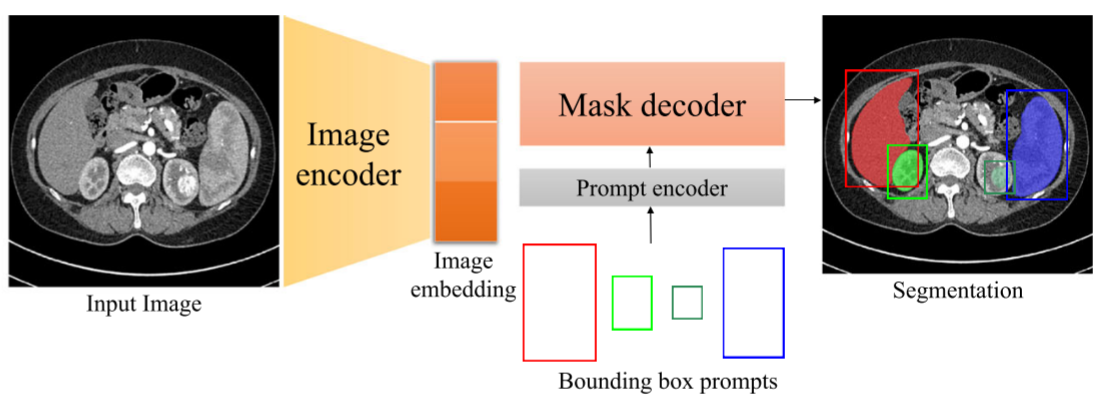
\includegraphics[width=\textwidth, height=.55\textheight]{./figures_ppt/MedSamModel.png}
      \caption{\label{fig:label}10.1038/s41467-024-44824-z }
    \end{figure}


  \end{column}
\end{columns}



% \textbf{Research Implication:} These models enable new paradigms for medyyical image analysis, particularly in \textbf{few-shot} and \textbf{zero-shot} learning scenarios where annotated data is scarce.
\end{frame}

\begin{frame}
  \frametitle{Foundation Models for Medical Image Segmentation}
  \framesubtitle{Segment Anything in Medical Images}
\begin{columns}
  \begin{column}{.5\textwidth}
    \begin{itemize}
      \item \textbf{Motivation:} To bridge the domain gap for medical
        imaging while retaining SAM's promptable, foundational design.
        \item \textbf{Approach:} Fine-tuned on a large-scale medical
          image dataset (over 1M masks from CT, MRI, ultrasound,
          etc.).
           \item \textbf{Key Advancement:} Enhances SAM's encoder with
             medical domain knowledge.
             \item \textbf{Significance:} No need to change model's
               architecture to specialize.
               \end{itemize}  
    
  \end{column}

  \begin{column}{.5\textwidth}
    \begin{figure}[ht]
      \centering
      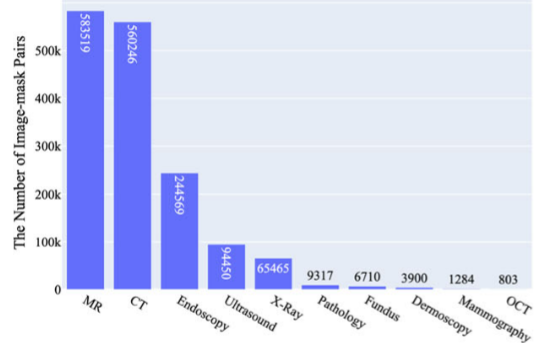
\includegraphics[width=\textwidth, height=.55\textheight]{./figures_ppt/MedSamTrainingData.png}
      \caption{\label{fig:label}10.1038/s41467-024-44824-z }
    \end{figure}


  \end{column}
\end{columns}



% \textbf{Research Implication:} These models enable new paradigms for medyyical image analysis, particularly in \textbf{few-shot} and \textbf{zero-shot} learning scenarios where annotated data is scarce.
\end{frame}

\subsection{Zero Shot Learning}

\begin{frame}
  \frametitle{Zero Shot Learning}

      \begin{itemize}

      \item Modern approach where a foundation model
        is used to predict and generalize to new data and new cases
        with no further training.
      \item Relies on a pre-trained model in a large dataset.
      \item In computer vision, it uses a visual prompt given by the
        user (i.e. human in the loop).
      \item It uses inference time.
      \item It exploits visual prompts with \ac{HITL}.
      \item It is a consequence of Transformer's \ac{OOD} capabilities.

      \end{itemize}



\end{frame}






% ===================================
% SECTION 2: METHODOLOGY
% ===================================
\section{Methodology}

% --- SLIDE 6: METHODOLOGY DETAILS ---
\begin{frame}
  \frametitle{Methodology Overview}
  \framesubtitle{ZSL with \ac{MedSAM}}

          \begin{enumerate}
  \item Select a sample dataset for manual labeling.
  \item Preprocess \ac{MG}s to remove artifacts.
  \item Generate Pectoral Muscle Masks using 5 different researchers.
  \item Generate Pectoral Muscle Masks using \ac{MedSAM}.
  \item Compute performance with segmentation scores.
  \end{enumerate}  
        
\end{frame}

\begin{frame}
  \frametitle{Methodology Overview}
  \framesubtitle{Otsu Algorithm Approach}

          \begin{itemize}
        \item Design a pipeline to apply Otsu's segmentation
          iteratively.
        \item Visually inspect Results
        \end{itemize}
\end{frame}

\subsection{MIAS Dataset Characteristics}


\begin{frame}{Dataset: Mammographic Image Analysis Society (MIAS)}
    The study utilizes the \textbf{Mini-MIAS database}, a standard benchmark for mammographic image analysis.


        \begin{itemize}
            \item \textbf{Source:} Digitized film mammograms (UK National Breast Screening Programme).
            \item \textbf{Volume:} 322 images from 161 patients.
            \item \textbf{View:} Medio-Lateral Oblique (MLO) view exclusively.
            \item \textbf{Resolution:} $1024 \times 1024$ pixels (PGM format).
            \item \textbf{Annotations:} Contains radiologist annotations for masses, calcifications, and asymmetries.
            \item \textbf{Format:} Approximate center coordinates ($x, y$) and radio ($r$) provided in \texttt{Info.txt}.
            % \item \textbf{Challenge:} Lack of pixel-wise segmentation masks necessitates the creation of the \textit{Human Reference Standard}.
        \end{itemize}

\end{frame}
% --- SLIDE 7: MODELS EVALUATED ---


\subsection{Experimental Procedure}


\begin{frame}[allowframebreaks]
  \frametitle{Experimental Design for \ac{ZSL}}
  \framesubtitle{Ground Truth Dataset} A total of 170 images from MIAS
  were randomly selected representing a 95\% confidence level with a
  5\% error.
  \begin{columns}
    \begin{column}{.5\textwidth}
      \begin{itemize}
        \item \textbf{Collaborative Annotation:} Dataset split among \textbf{5 independent researchers}.
        \item \textbf{Annotation Tools:}
        \begin{itemize}
            \item Manual Polygon delineation.
            \item Superpixel segmentation for boundary adherence.
        \end{itemize}
        \item \textbf{Refinement:} Applied morphological operations
          (\textit{Dilation} and \textit{Erosion}).
        \item \textbf{Output:} 
        \begin{itemize}
            \item Mask A: Pectoral Muscle.
            \item Mask B: Glandular Tissue.
        \end{itemize}
      \end{itemize}
      
      
    \end{column}

    \begin{column}{.5\textwidth}
      \begin{figure}[ht]
        \centering
        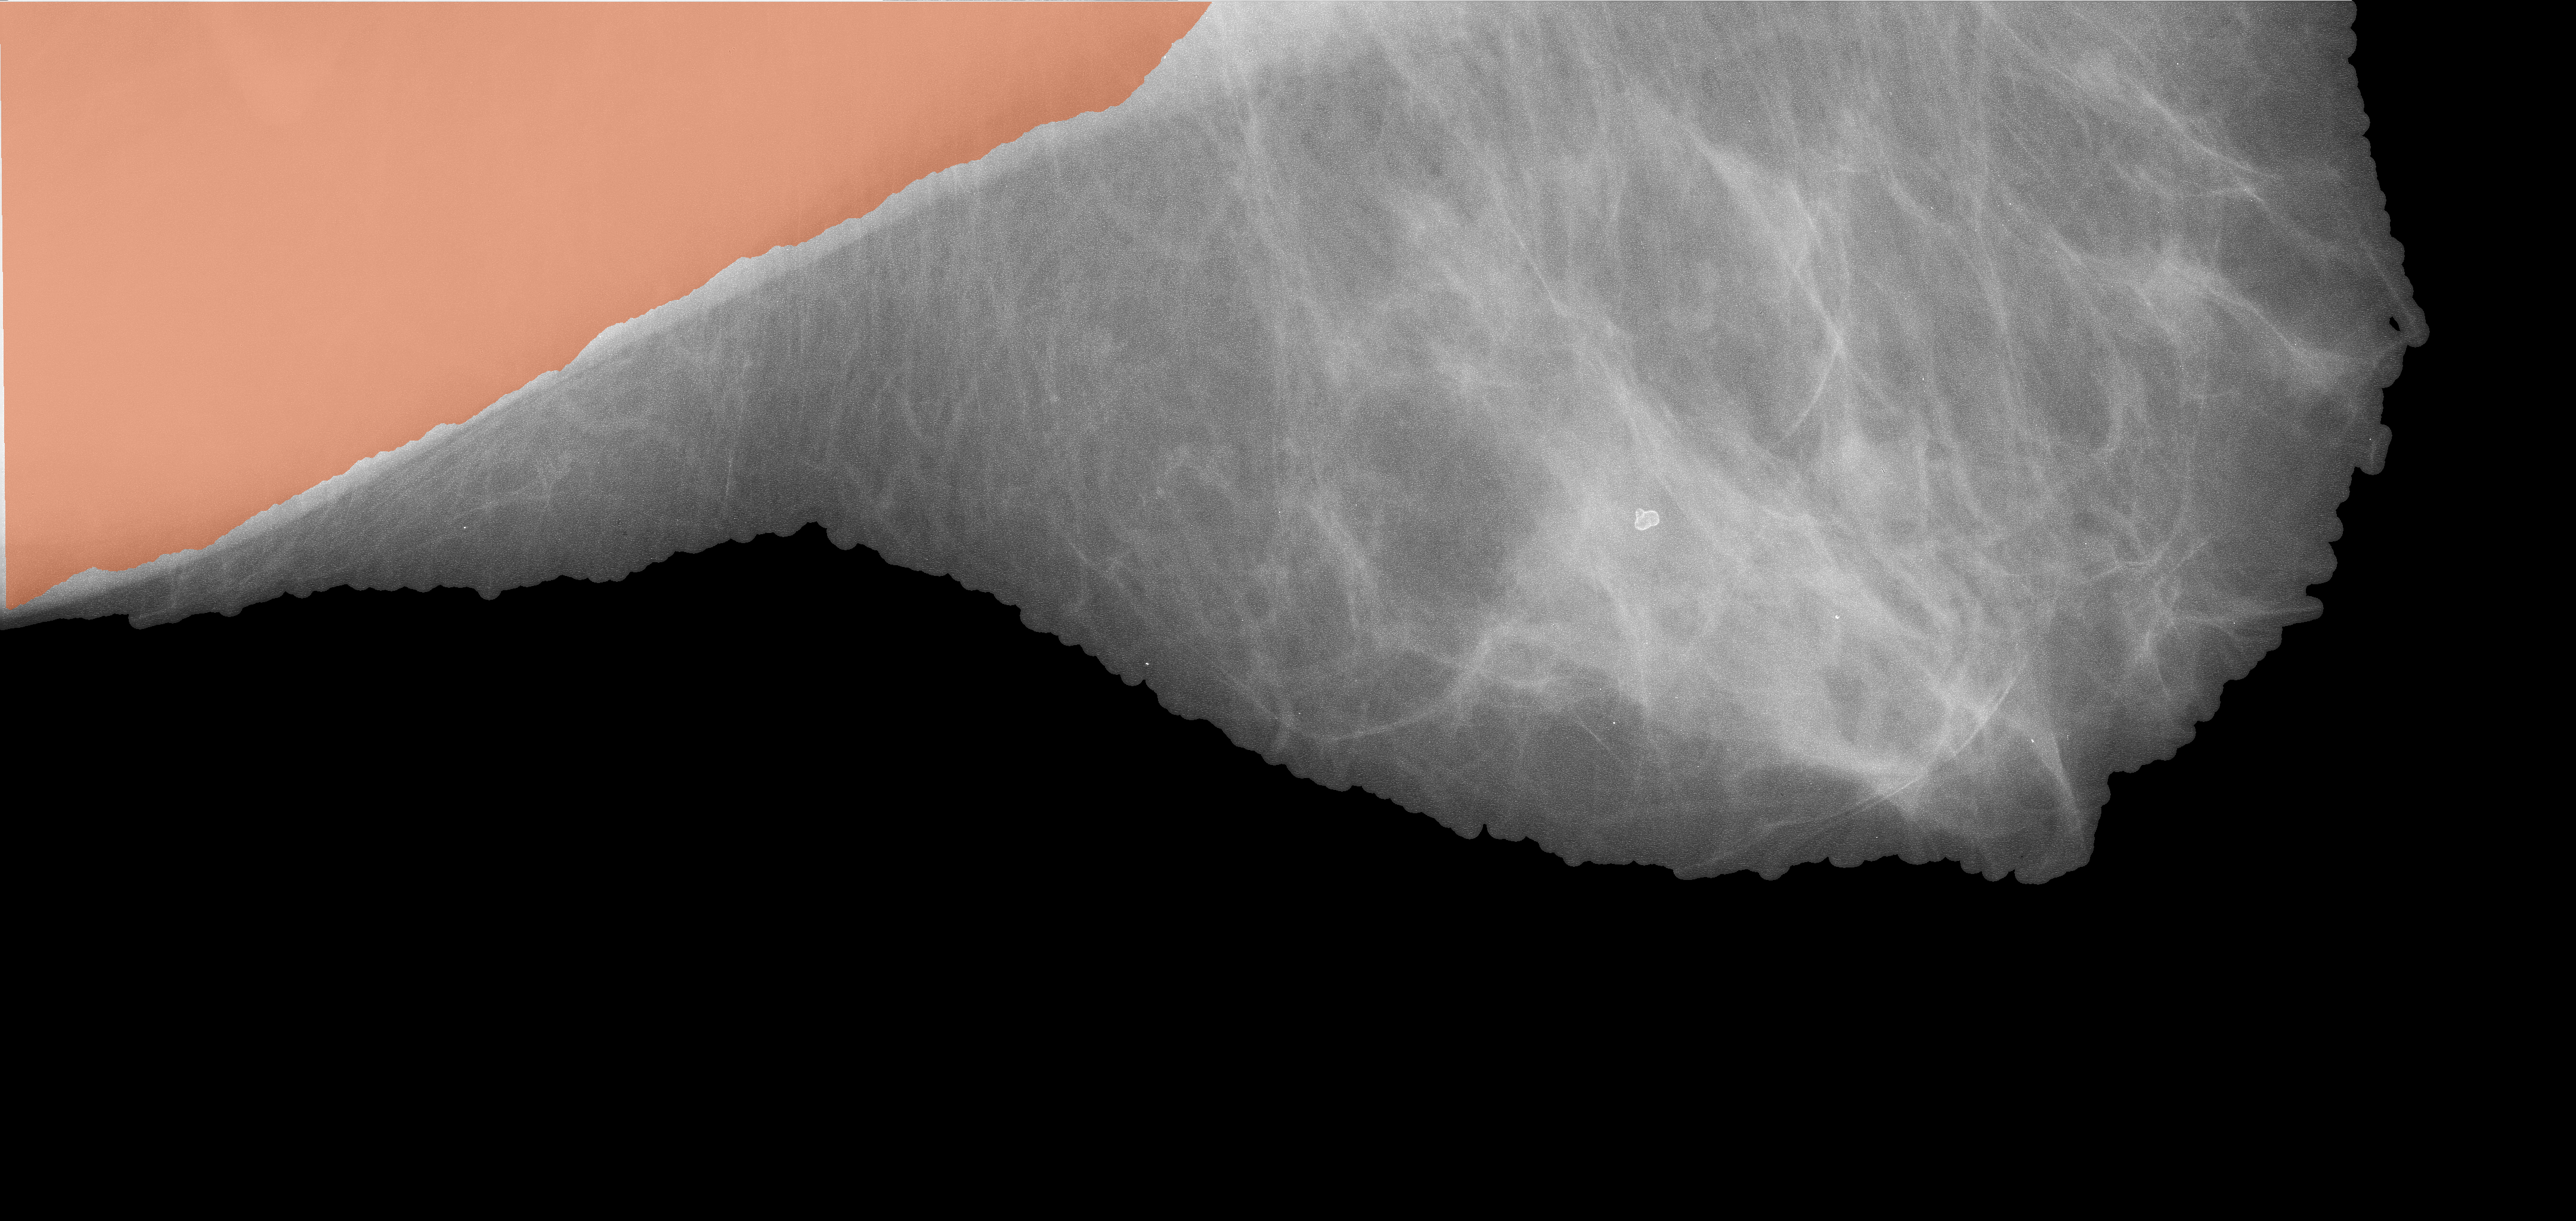
\includegraphics[width=\textwidth, height=.6\textheight]{./figures_ppt/case48_GT.png}
        \caption{\label{fig:label}Ground Truth for case 48 }
      \end{figure}


    \end{column}
  \end{columns}

  % \begin{figure}[ht]
  %   \centering
  %   
\includegraphics[width=\textwidth, height=.7\textheight]{../figures/experimentalMethodologyGuide.png}
  %   \caption{\label{fig:label} Guide for experimental procedure with
  %     results in F1-score}
  % \end{figure}

\end{frame}

\begin{frame}
  \frametitle{Experimental Design for \ac{ZSL}}
  \framesubtitle{\ac{MedSAM}'s predicted dataset}
  \begin{columns}
    \begin{column}{.5\textwidth}
        
 \begin{enumerate}
            \item \textbf{Integration:} Loaded MedSAM model directly into Medical Image Labeler.
            \item \textbf{Prompting Strategy:} Used a \textbf{Bounding Box} prompt covering the pectoral muscle area.
            \item \textbf{Anchor Point:} Box initiation started from the upper edge where the muscle originates.
            \item \textbf{Selection:} Multiple prompts were tested;
              the result with the highest visual fidelity was
              selected.
            \item No further operations (dilation or erosion) were allowed.
        \end{enumerate}
 
      
    \end{column}

    \begin{column}{.5\textwidth}
\begin{figure}[ht]
  \centering
  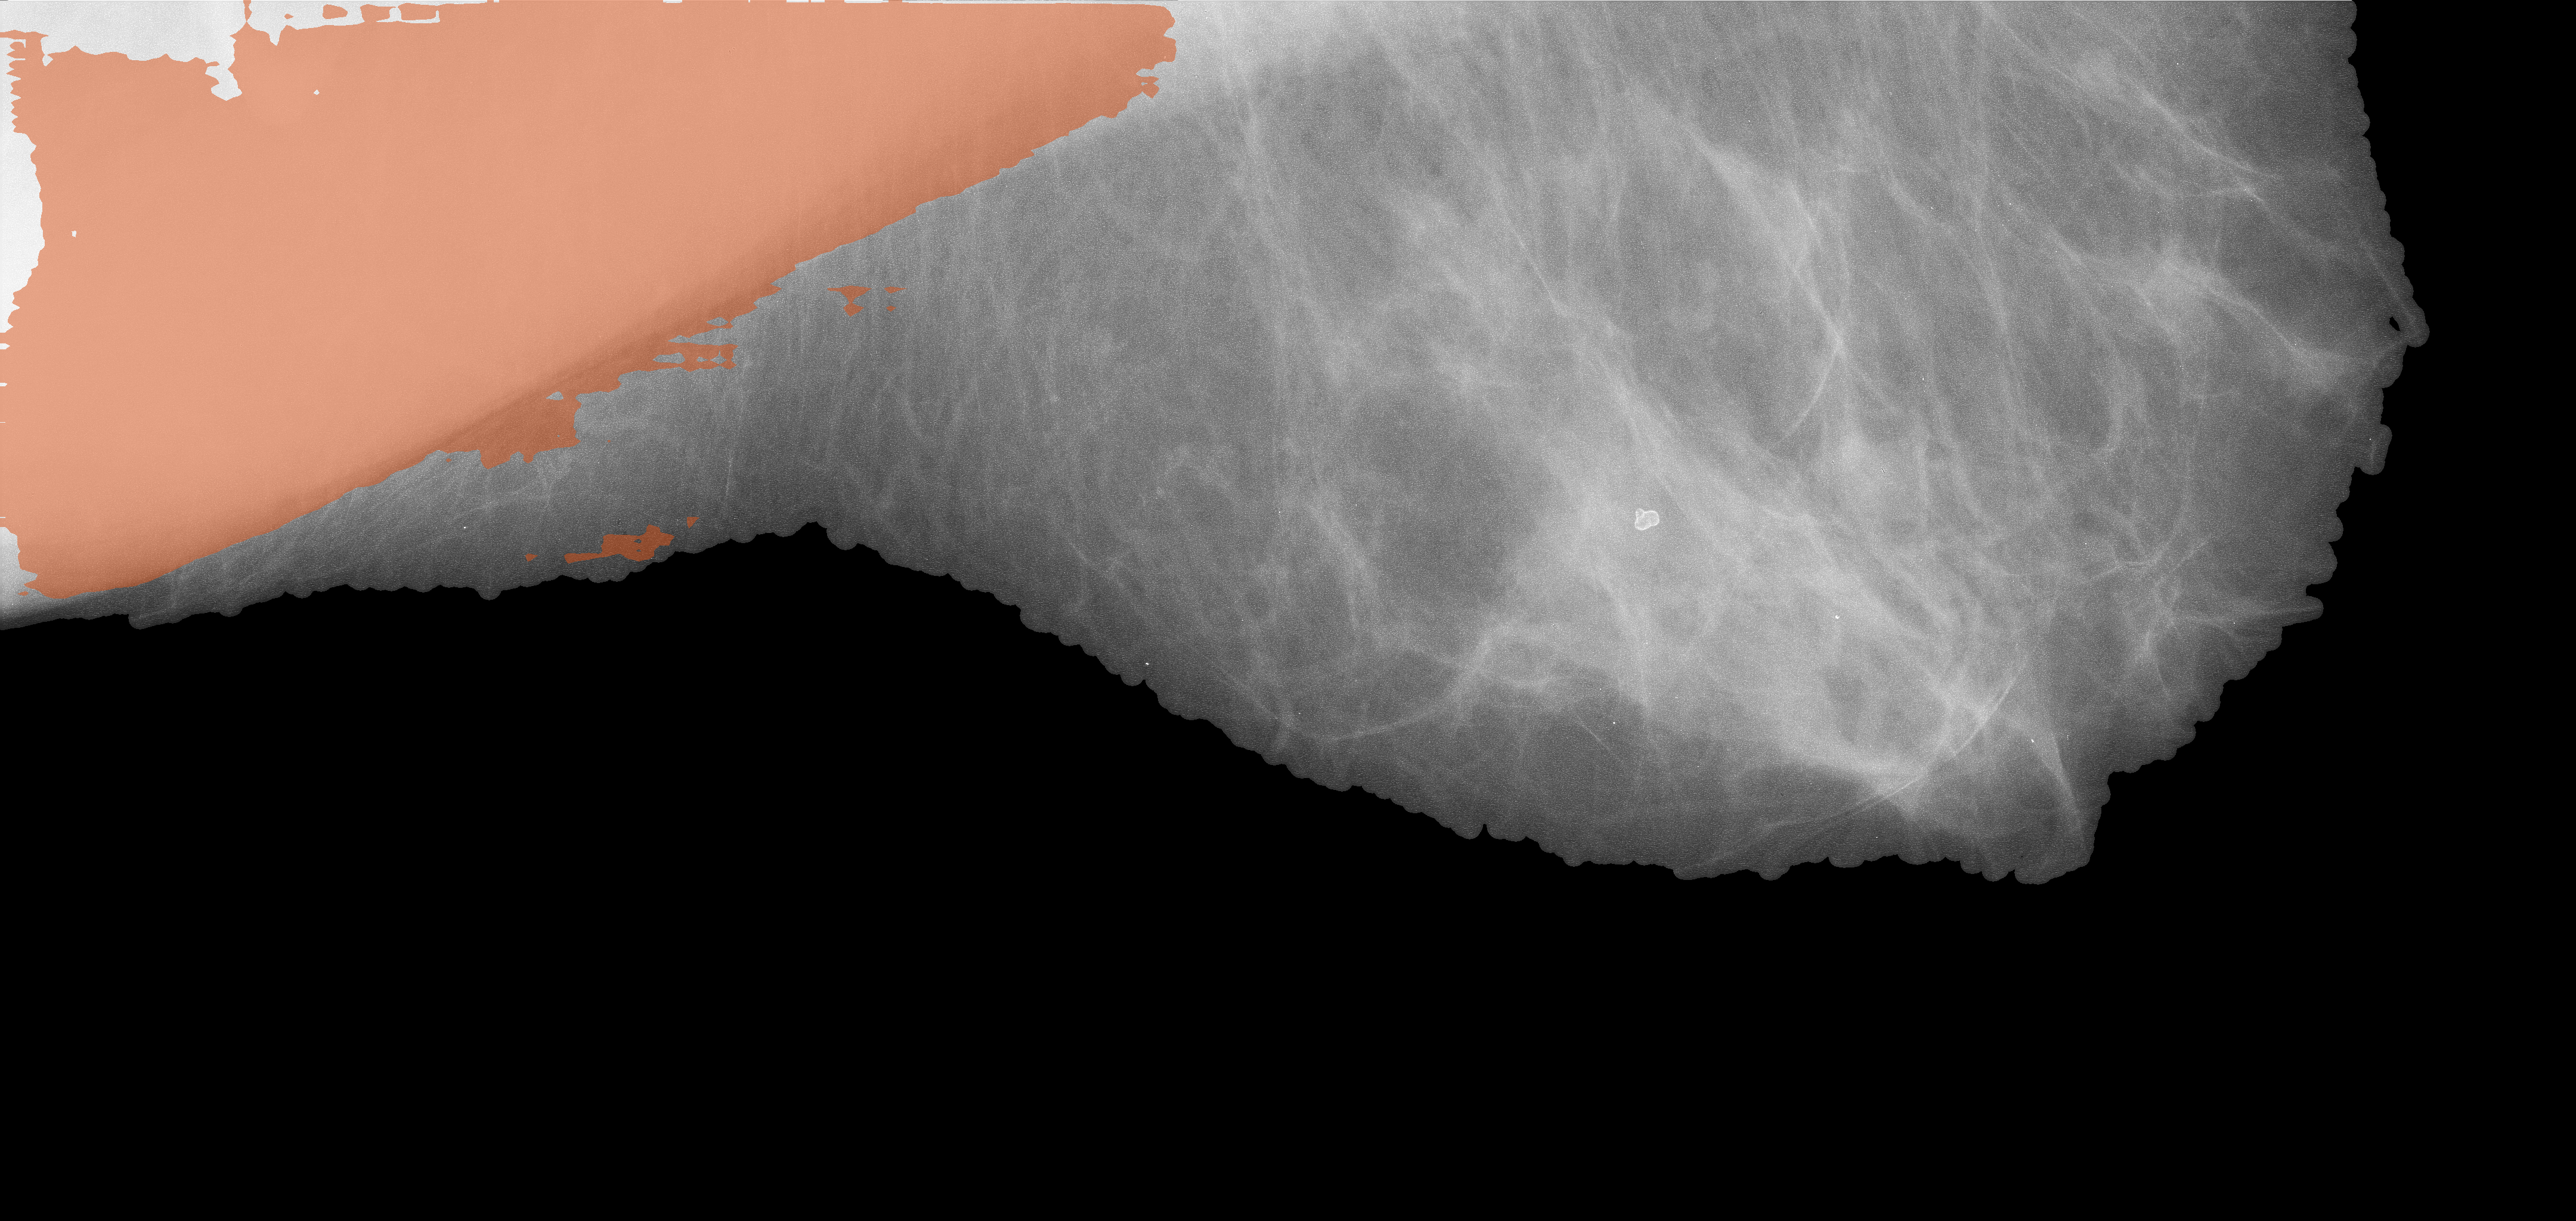
\includegraphics[width=\textwidth, height=.6\textheight]{./figures_ppt/case48_medSAM.png}
  \caption{\label{fig:label}MedSAM prediction of case 48 }
\end{figure}

    \end{column}
  \end{columns}

\end{frame}

% --- Slide 1 ---
\begin{frame}{Global Otsu Threshold}
\begin{itemize}
    \item Normalize the image intensities to the range $[0,1]$:
    \[
    I_0 = \frac{I_{\text{raw}} - \min(I_{\text{raw}})}{\max(I_{\text{raw}} - \min(I_{\text{raw}}))}
    \]
    \item Apply Otsu’s method to compute the global threshold $T_1$.
    \item Otsu selects $T_1$ that maximizes the between-class variance:
    \[
    \sigma_B^2(T) = \omega_0(T)\,\omega_1(T)\,[\mu_0(T) - \mu_1(T)]^2
    \]
    \item This separates the image into two main regions: \textbf{low} ($I_0 < T_1$) and \textbf{high} ($I_0 \geq T_1$).
\end{itemize}
\end{frame}

% --- Slide 2 ---
\begin{frame}{Subdivision into Four Classes}
\begin{itemize}
    \item Apply Otsu again within each subset:
    \[
    T_{\text{low}} = \text{Otsu}(I_0 \mid I_0 < T_1), \quad
    T_{\text{high}} = \text{Otsu}(I_0 \mid I_0 \geq T_1)
    \]
    \item If subsets are empty, use defaults: $T_{\text{low}} \approx T_1/2$, $T_{\text{high}} \approx (1+T_1)/2$.
    \item Final segmentation into four regions:
    \[
    \begin{aligned}
    \text{Class 1: } & I_0 < T_{\text{low}} \\
    \text{Class 2: } & T_{\text{low}} \leq I_0 < T_1 \\
    \text{Class 3: } & T_1 \leq I_0 < T_{\text{high}} \\
    \text{Class 4: } & I_0 \geq T_{\text{high}}
    \end{aligned}
    \]
    % \item Produces a label map with values $\{1,2,3,4\}$.
\end{itemize}
\end{frame}
% ===================================
% SECTION 3: RESULTS
% ===================================
\section{Results}
\begin{frame}{Performance Evaluation Metrics of MedSAM}
    To quantify the inter-method agreement between the Zero-Shot MedSAM predictions ($P$) and the Human Reference Standard ($G$):

    \begin{block}{Volumetric Agreement}
        \begin{equation*}
            \text{Dice Coefficient (DSC)} = \frac{2 |P \cap G|}{|P| + |G|}
        \end{equation*}
        \begin{equation*}
            \text{Intersection over Union (IoU)} = \frac{|P \cap G|}{|P \cup G|}
        \end{equation*}
    \end{block}

    \vspace{0.2cm}
    \textbf{Additional Metrics:} Precision and  Recall were calculated to assess over-segmentation and boundary adherence.
  \end{frame}

\begin{frame}
  \frametitle{Performance Evaluation of MedSAM}
  % \begin{figure}[ht]
    \centering
    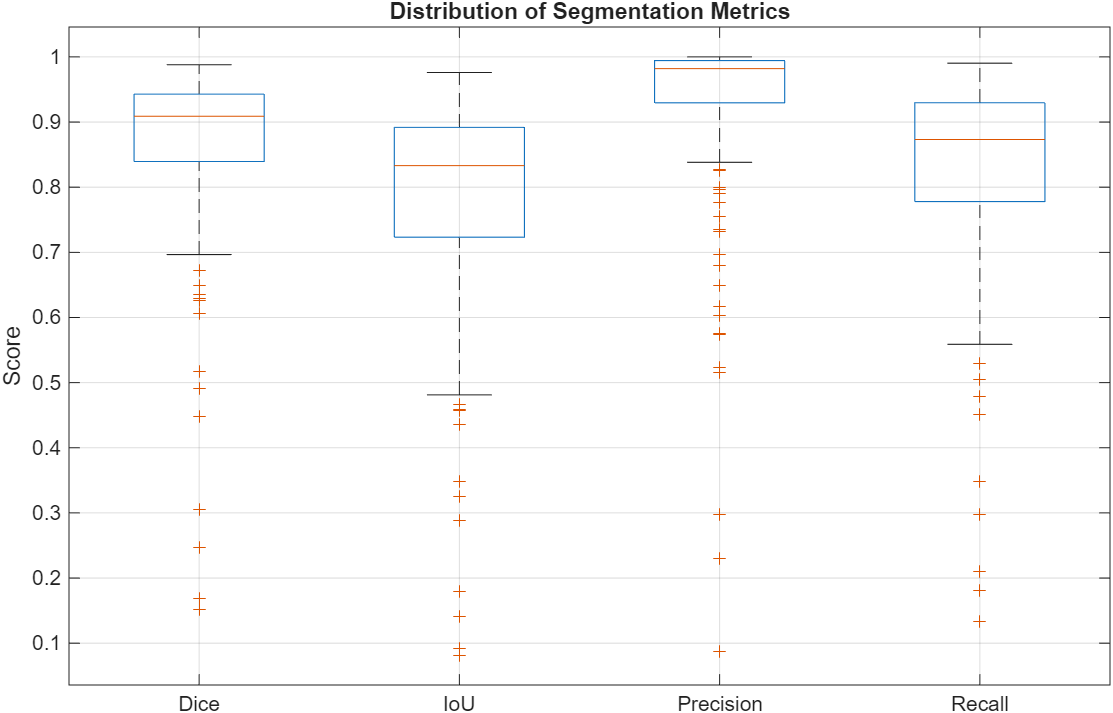
\includegraphics[width=\textwidth, height=.6\textheight]{./figures_ppt/SegmentationMetricsPerformance.png}
  %   \caption{\label{fig:label} }
  % \end{figure}

  \end{frame}

  \begin{frame}
  \frametitle{Performance Evaluation of MedSAM}
  % \begin{figure}[ht]
    \centering
    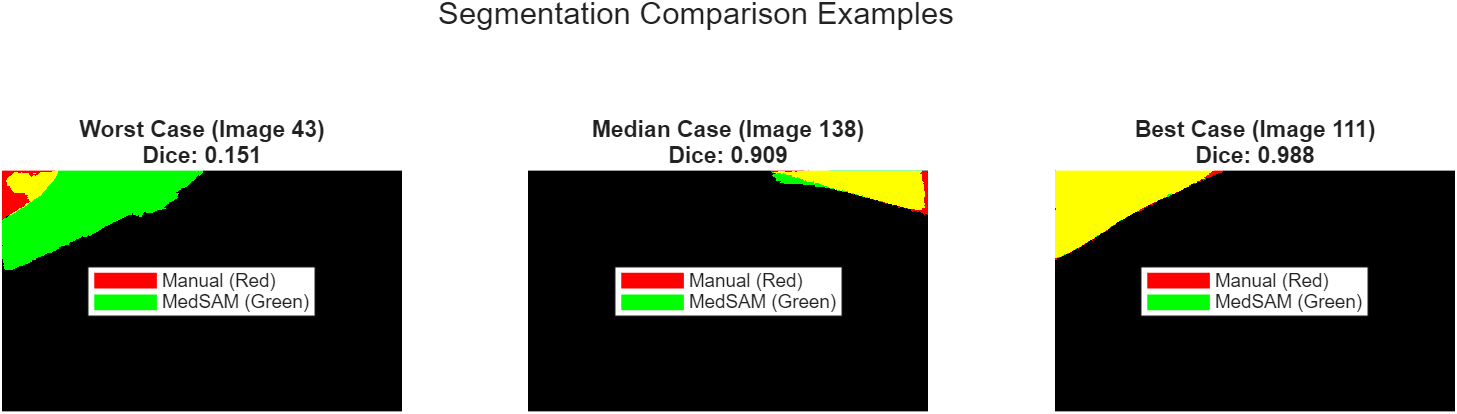
\includegraphics[width=\textwidth, height=.6\textheight]{./figures_ppt/SegmentationComparisonExamples_withLegend.png}
  %   \caption{\label{fig:label} }
  % \end{figure}

  \end{frame}

% \begin{frame}
%   \frametitle{Performance Evaluation of MedSAM}
%   \begin{itemize}
%     \item \textbf{Dice Score:} \\
%     Mean = 0.865 $\pm$ 0.140, \quad Median = 0.909
%     \item \textbf{Jaccard (IoU):} \\
%     Mean = 0.783 $\pm$ 0.171, \quad Median = 0.833
%     \item \textbf{Precision:} \\
%     Mean = 0.925 $\pm$ 0.141, \quad Median = 0.982
%     \item \textbf{Recall:} \\
%     Mean = 0.830 $\pm$ 0.151, \quad Median = 0.873
% \end{itemize}
  
% \end{frame}


\begin{frame}
  \frametitle{Performance Evaluation of MedSAM}
\centering
\begin{tabular}{lccccc}
\hline
\textbf{Metric} & \textbf{Mean} & \textbf{Std} & \textbf{Median} & \textbf{Min} & \textbf{Max} \\
\hline
Dice      & 0.86531 & 0.14039 & 0.90895 & 0.15112  & 0.98791 \\
IoU       & 0.78329 & 0.17118 & 0.83310 & 0.08174  & 0.97611 \\
Precision & 0.92517 & 0.14076 & 0.98206 & 0.08738  & 1.00000 \\
Recall    & 0.82970 & 0.15068 & 0.87316 & 0.13349  & 0.99039 \\
\hline
\end{tabular}

  
\end{frame}

\begin{frame}
  \frametitle{Iterative Otsu}
    \centering
    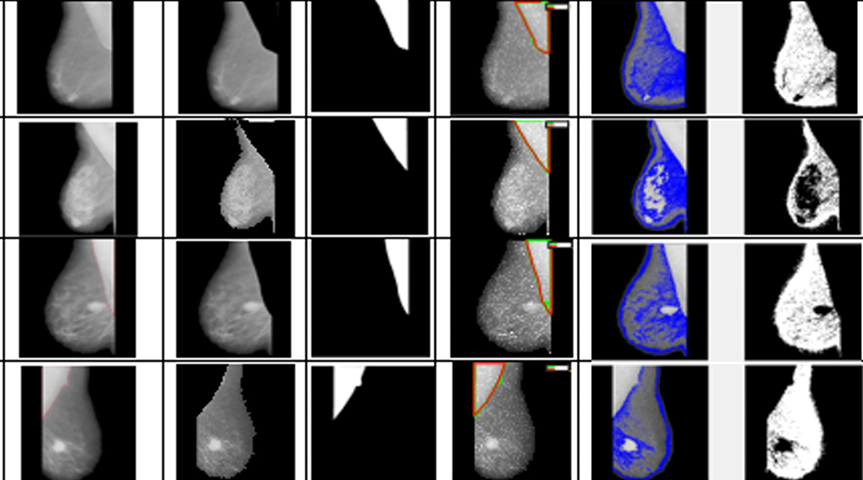
\includegraphics[width=\textwidth, height=.6\textheight]{./figures_ppt/otsus_result.png}
  
\end{frame}


% ===================================
% SECTION 4: CONCLUSION
% ===================================
\section{Conclusion}

% --- SLIDE 11: CONCLUSION ---
\begin{frame}[allowframebreaks]
  \frametitle{Conclusion}
\begin{itemize}

\item \ac{ZSL} with foundation model such as \ac{MedSAM} can aid in
  pectoral muscle segmentation.
  Score.
\item MedSAM presented a performance near 0.90 for Dice Score without
  further training.
\item Foundation Models can be used to aid in labeling operations for
  medical data.
\item Traditional approaches, such Otsu's iteratively, present
  relevant results and do not need high computational resources
  compared to Transformer-based models and work independent of \ac{MG}
  orintation.
\item Iterative Otsu needs an additional step to separate muscle from
  mass. It can be hybrid by using a foundation model or calculating
  the size of the areas.
\end{itemize}
\end{frame}

\begin{frame}
  \frametitle{Limitations and Future Work}
  \begin{itemize}
  \item \textbf{Dataset Scope:} This study utilized a subset of the \ac{MIAS} dataset. Future work should validate our approach on the complete \ac{MIAS} dataset and extend evaluation to additional public mammography datasets.
  \item \textbf{Annotation Process:} Ground truth annotations were obtained from individual radiologists. Future studies should implement consensus labeling or multiple annotator review to assess and mitigate potential labeling bias.
  \item \textbf{Human-in-the-Loop Refinement:} The integration of \ac{HITL} mechanisms for prompt refinement requires further investigation to quantify and control for introduced human biases in the interactive learning process.
  \end{itemize}
\end{frame}
% --- SLIDE 12: Q&A ---
\begin{frame}
  \frametitle{Q\&A} % No title
  \begin{columns}
    \begin{column}{.5\textwidth}
        \centering
  \Huge
  Thank You
  \vspace{1em}
  \Large
  Questions?\\
      
    \end{column}

    \begin{column}{.5\textwidth}
      \centering
      \Large
      Lenin G. Falconi: \\
      
\includegraphics[width=\textwidth]{./figures_ppt/linkedin3.png}
      lenin.falconi@epn.edu.ec

    \end{column}
  \end{columns}

\end{frame}
% Bibliography
% \begin{frame}[allowframebreaks]
%     \frametitle{References}
%     % \nocite{*} % This command will include all entries from your .bib file
%     \printbibliography
% \end{frame}
\end{document}


%%% Local Variables:
%%% mode: LaTeX
%%% TeX-master: t
%%% End:
